\subsubsection{データベースのテーブルの作成}
データベースはSQLite3を用いることが決まっていたため、コマンドラインからテーブルの作成を行えたが、本チームではGUIのデータベース管理ソフト「Lita」を用いることにした。このLitaはWindowsやMac等のOS環境に依存せず、データの挿入や問い合わせ作業が単純であるため、データベースの状態を確認したい時に効率が良いと考えた。図\ref{fig:lita}はテーブルの作成に用いたデータベース管理ソフト、Litaの利用図である。

 \begin{figure}[h]
 \centering
 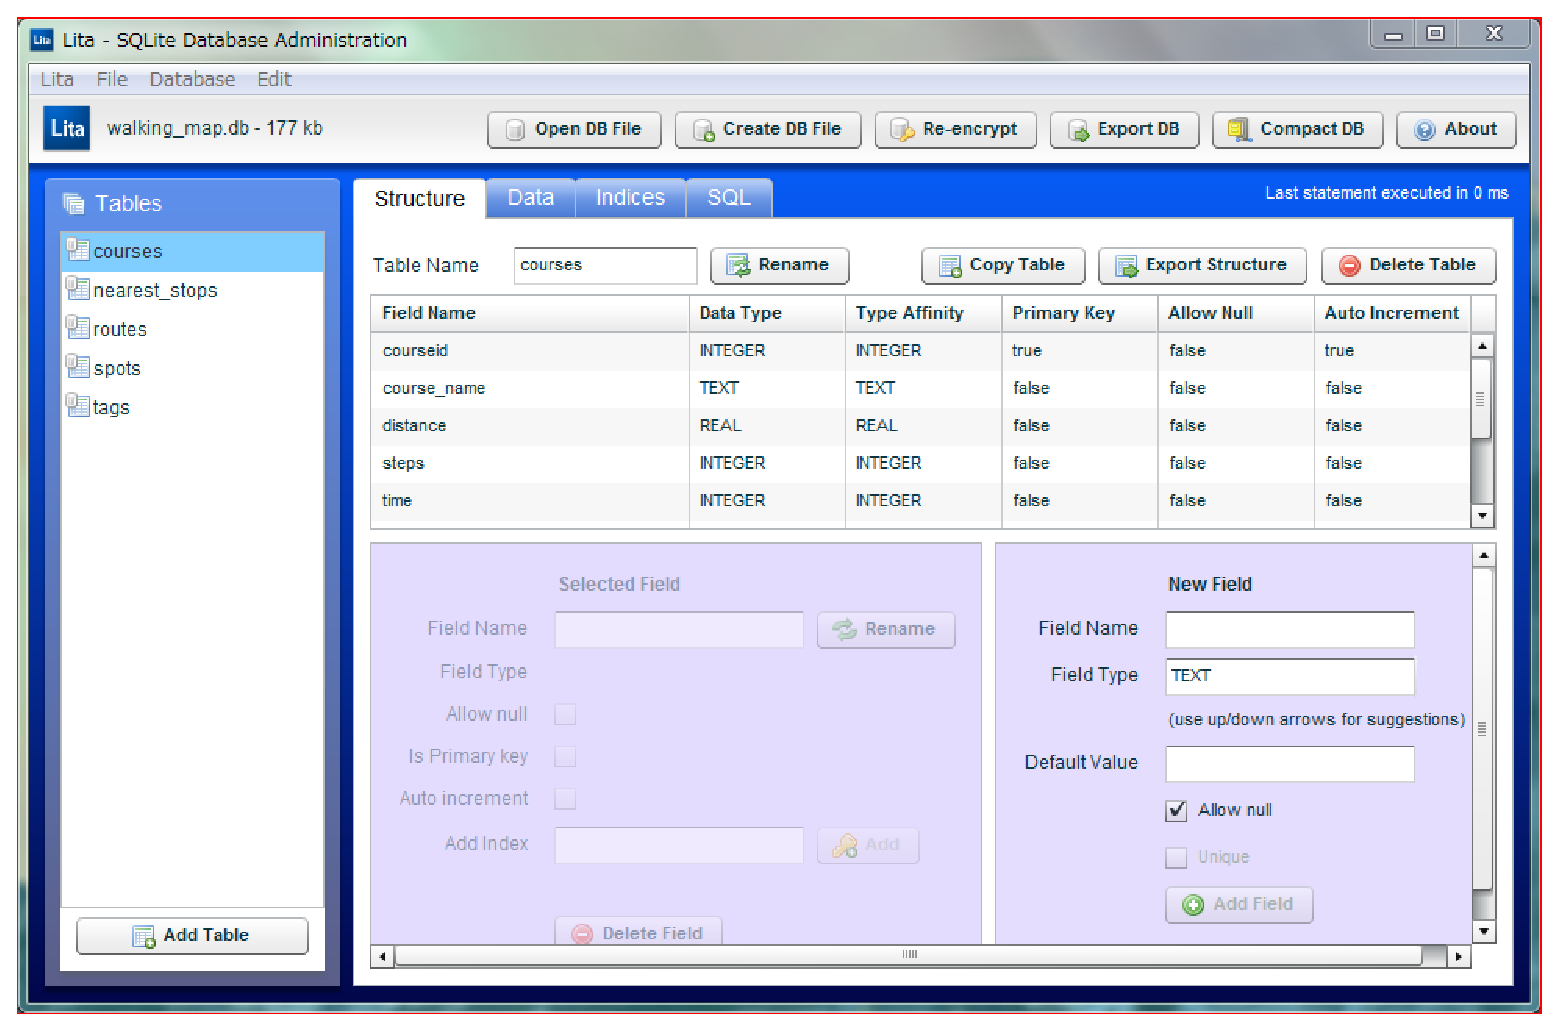
\includegraphics[scale=0.38]{lita.eps}
 \caption{テーブルの作成に用いたデータベース管理ソフト「Lita」}
 \label{fig:lita}
 \end{figure}

 \bunseki{仲松聡}
